% XeLaTeX

\documentclass{article}
\usepackage{ctex}
\usepackage{xypic}
\usepackage{amsfonts,amssymb}
\usepackage{multirow}
\usepackage{geometry}
\usepackage{graphicx}
\usepackage{listings}
\usepackage{lipsum}
\usepackage{courier}
\usepackage{fancyvrb}
\usepackage{etoolbox}


\linespread{1.2}
\geometry{left=3cm,right=2.5cm,top=2.5cm,bottom=2.5cm}

\makeatletter
\patchcmd{\FV@SetupFont}
  {\FV@BaseLineStretch}
  {\fontencoding{T1}\FV@BaseLineStretch}
  {}{}
\makeatother

\lstset{basicstyle=\small\fontencoding{T1}\ttfamily,breaklines=true}
\lstset{numbers=left,frame=shadowbox,tabsize=4}
%\lstset{extendedchars=false}
\begin{document}

\title{实验七 \ 父子进程通信 \ 实验报告}
\author {数据科学与计算机学院 \ 计算机科学与技术 2016 级 \\ 王凯祺 \ 16337233}
\maketitle

\section{实验目的}

\begin{itemize}
\item 进一步完善进程模型,建立一组合作进程,并发运行,各自完成一定的工作。
\item 理解并实现操作系统的 fork, wait, exit 机制。
\end{itemize}

\section{实验要求}

在实验六的原型基础上,进化我的原型操作系统,原型保留原有特征的基础上,设计满足下列要求的新原型操作系统:

\begin{itemize}
\item 实现控制的基本原语 do\_fork() 、do\_wait() 、 do\_exit() 、 blocked() 和 wakeup() 。
\item 内核实现三系统调用 fork() 、 wait() 、 exit() ,并在 C 库中封装相关的系统调用。
\item 编写一个 C 语言程序,实现多进程合作的应用程序。
\end{itemize}

\section{实验步骤}

\subsection{设计思路}

首先,我认为一个进程的状态只需要四种状态就可以表示:死亡(创建前和退出后均视为死亡)、就绪、运行、阻塞,而不需要五种状态。

对于进程创建 fork() 、进程退出 exit() 和父子进程通信 wait() ,应用中断调用中断服务程序。这三个中断服务程序应在内核实现,它们通过修改进程控制块,从而达到上述目的。

\subsection{扩展进程控制块}

由于将二进程模型升级为五进程模型,进程控制块的修改是必要的。我们应新增以下数据项:

\begin{itemize}
\item status 表示当前进程的状态(0 表示死亡, 1 表示就绪, 2 表示运行, 3 表示阻塞)。
\item father\_pid 表示父进程的 pid 。
\item son\_cnt 表示有多少个\textbf{直接的}子进程。
\item ret\_val 表示\textbf{最后一个}退出的子进程的返回值。
\end{itemize}

\begin{lstlisting}[language=C]
typedef struct PCB {
	int ax;
	int bx;
	int cx;
	int dx;
	int si;
	int di;
	int bp;
	int es;
	int ds;
	int ss;
	int sp;
	int ip;
	int cs;
	int flags;
	int status;
	int father_pid;
	int son_cnt;
	int ret_val;
	char pname[16];
};

const int DEAD = 0;
const int READY = 1;
const int RUNNING = 2;
const int BLOCK = 3;

int now_process;
\end{lstlisting}

PCBlist 的下标即代表进程号,这个进程号不再是磁盘扇区的编号,较上个实验有改进。这样就支持同一个程序创建多个进程。

\subsection{编写 C 语言测试程序}

既然老师写好了,那我就直接拿来用好啦!

\begin{lstlisting}[language=C++]
/* forkmain.c */

#include "process.h"
#include "forkio.h"

char str[55] = "129djwqhdsajd128dw9i39ie93i8494urjoiew98kdkd";

int LetterNr = 0;

void forkmain() {
	int pid, i, j;
	int ch;
	pid = fork();
	if (pid == -1) puts_no_new_line("error in fork!\n");
	if (pid) {
		puts_no_new_line("child pid=");
		printint(pid);
		ch = wait();
		puts_no_new_line("return val=");
		printint(ch);
		for (i = 0; str[i]; ++i);
		puts_no_new_line("tot len=");
		printint(i);
		exit(0);
	} else {
		j = 0;
		for (i = 0; str[i]; ++i)
			if (str[i] >= 'a' && str[i] <= 'z')
				++ j;
		puts_no_new_line("alpha len=");
		printint(j);
		exit(0);
	}
}
\end{lstlisting}

process.h 就是调用中断的库。

\begin{lstlisting}[language=C++]
/* process.h */
void exit(int ret_val) {
	char tmp;
	tmp = ret_val;
	asm mov ah, 4ch
	asm mov al, tmp
	asm int 21h
}

int fork() {
	asm int 22h
}

int wait() {
	asm int 23h
}
\end{lstlisting}

\subsection{进程创建 forkint 原语}

我思考了一下, forkint 原语要做的事情有很多啊!

\begin{itemize}
\item 执行 Save 过程,保存当前进程状态。
\item 在 PCB 表查找空闲表项,若找不到空闲表项,将 $ax$ 置为 $-1$ ,执行 Restart 过程。
\item 若找到空闲表项,将父进程的 PCB 复制给子进程。
\item 将父进程所使用的代码段、数据段、堆栈段全部复制给子进程。
\item 修改子进程的 cs 、 ds 、 es 、 ss 。
\item 激活子进程,将其设置为就绪状态。
\item 分别设置 fork() 函数的返回值,该步骤只需将对应的进程控制块中 $ax$ 的值修改即可。
\item 执行 Restart 过程。
\end{itemize}

好,那就一个个做啦!

首先先用汇编写 loader ,中断向量首先指向 loader ,然后 loader 再调用 C ,执行其他语句块。

\paragraph{fork 中断 loader}

我将 fork 设置为 22h 号中断,用户程序通过中断调用来实现 fork 。

\begin{lstlisting}[language={[x86masm]Assembler}]
extrn _forkint:near

forkint:
	cli
	call near ptr Save
	
	mov ax, 0a00h
	mov ds, ax
	mov es, ax
	mov ss, ax
	mov sp, 0h
	call near ptr _forkint
	call near ptr Restart
\end{lstlisting}

\paragraph{forkint 过程}

这一部分用 C 语言写,下面这段代码应该非常地简单易懂啦!

\begin{lstlisting}[language=C++]
void forkint() {
	int tmp;
	save();
	tmp = find_dead_process();
	if (tmp == -1) {
		new_pcb.ax = -1;
		PCBcopy(&PCBlist[now_process], &new_pcb);
	} else {
		ProcessCopy(0x2000 + 0x40 * tmp, 0x2000 + 0x40 * now_process);
		new_pcb.ax = tmp;
		PCBcopy(&PCBlist[now_process], &new_pcb);
		PCBlist[now_process].son_cnt += 1;
		new_pcb.ax = 0;
		new_pcb.cs += (tmp - now_process) * 0x40;
		new_pcb.ds += (tmp - now_process) * 0x40;
		new_pcb.es += (tmp - now_process) * 0x40;
		new_pcb.ss += (tmp - now_process) * 0x40;
		PCBcopy(&PCBlist[tmp], &new_pcb);
		PCBlist[tmp].father_pid = now_process;
		make_alive(tmp);
	}
	restore(now_process);
}
\end{lstlisting}

\subsection{进程终止 exit 原语}

exit 原语要做的事情有:

\begin{itemize}
\item 修改进程控制块,结束进程。
\item 更新父进程信息,解除阻塞。
\item jmp \$
\end{itemize}

最后一条要解释一下,做完前两个步骤后,CPU 的控制权仍在这个进程手上,而且 CPU 不会再次把控制权交给这个进程。所以我采用死循环的方式,等待时钟中断来临时将 CPU 控制权夺去,从而结束该进程。


同样地,先用汇编写 loader ,中断向量首先指向 loader ,然后 loader 再调用 C ,执行其他语句块。

\paragraph{exit 中断 loader}

我将 exit 设置为 21h 号中断 4C 功能号,与 DOS 一致。用户程序通过中断调用来实现 exit 。

\begin{lstlisting}[language={[x86masm]Assembler}]
extrn _dosint:near

dosint:
	push ds
	push es
	push ax
	mov ax, 0a00h
	mov ds, ax
	mov es, ax
	pop ax
	call near ptr _dosint
	pop es
	pop ds
	iret
\end{lstlisting}

\paragraph{exitint 过程}

这一部分用 C 语言写,下面这段代码应该非常地简单易懂啦!

\begin{lstlisting}[language=C++]
void dosint() {
	char tah, tal;
	int tax;
	asm mov tah, ah
	asm mov tal, al
	asm mov tax, ax
	if (tah == 0x4c) {
		asm cli
		kill_pid(now_process, tal);
		asm sti
		asm jmp $
	}
}
\end{lstlisting}

顺便再贴一个 kill\_pid 的代码,体现了对父进程的操作,包括解除阻塞、设置返回值等……

\begin{lstlisting}[language=C++]
void kill_pid(int pid, int ret_val) {
	int j;
	if (pid == 0) return;
	if (PCBlist[pid].status == DEAD) return;
	PCBlist[pid].status = DEAD;
	PCBlist[PCBlist[pid].father_pid].son_cnt -= 1;
	if (PCBlist[PCBlist[pid].father_pid].son_cnt == 0 &&
		PCBlist[PCBlist[pid].father_pid].status == BLOCK) {
		PCBlist[PCBlist[pid].father_pid].status = READY;
		PCBlist[PCBlist[pid].father_pid].ax = ret_val;
	}
	PCBlist[PCBlist[pid].father_pid].ret_val = ret_val;
	for (j = 0; j < 64; ++j)
		if (PCBlist[j].status != DEAD && PCBlist[j].father_pid == pid) {
			PCBlist[j].father_pid = 0;
			PCBlist[pid].son_cnt -= 1;
			PCBlist[0].son_cnt += 1;
		}
}
\end{lstlisting}

\subsection{进程等待子进程结束 wait 原语}

wait 原语要做的事情有:

\begin{itemize}
\item 执行 Save 过程。
\item 如果当前有儿子进程正在运行,则阻塞当前进程;若没有,将最后一个结束的子进程的返回值写入 $ax$ 寄存器中。
\item 执行 Schedule 过程。
\item 执行 Restart 过程。
\end{itemize}

首先先用汇编写 loader ,中断向量首先指向 loader ,然后 loader 再调用 C ,执行其他语句块。

\paragraph{wait 中断 loader}

我将 wait 设置为 23h 号中断,用户程序通过中断调用来实现 wait 。

\begin{lstlisting}[language={[x86masm]Assembler}]
extrn _waitint:near

waitint:
	cli
	call near ptr Save
	
	mov ax, 0a00h
	mov ds, ax
	mov es, ax
	mov ss, ax
	mov sp, 0h
	call near ptr _waitint
	call near ptr Restart
\end{lstlisting}

\paragraph{waitint 过程}

这一部分用 C 语言写,下面这段代码应该非常地简单易懂啦!

\begin{lstlisting}[language=C++]
void waitint() {
	save();
	if (PCBlist[now_process].son_cnt > 0)
		PCBlist[now_process].status = BLOCK;
	else
		new_pcb.ax = PCBlist[now_process].ret_val;
	exchange();
}
\end{lstlisting}

\paragraph{遇到的问题}

写完上面的三个原语之后,就可以拿去虚拟机测试了!

不出所料,肯定是不正常的……

\begin{figure}[!hbp]
	\centering
	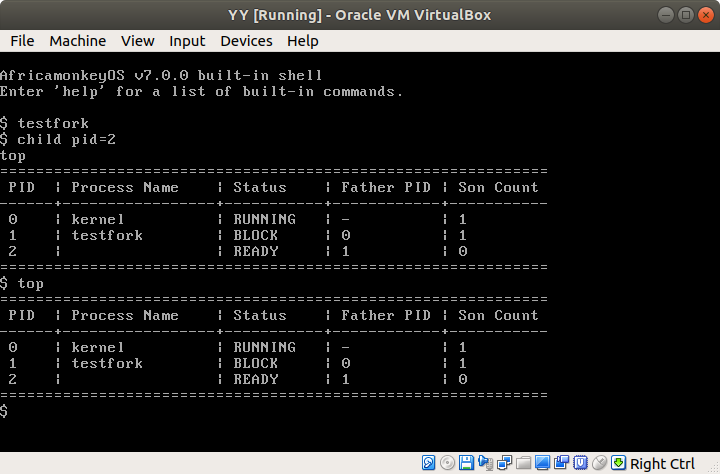
\includegraphics[scale=0.55]{pics/1.png}
\end{figure}

利用之前写的 top 命令,我们可以看到,测试程序成功执行 fork 命令,父进程能成功得到子进程 pid 。父进程执行到 wait 命令时,成功被阻塞,却再也出不来了,产生了死锁。

我们还能看到,除了父进程有输出以外,屏幕上只有子进程的进程控制块,却没有它输出的任何信息。

据此可以判断,子进程没有被成功执行,应该是 fork 的时候错了。

仔细检查 fork 的代码,并没有错,符合我的思维逻辑。这样的话,只能进 bochs 跟踪了……

我把断点设置在时钟中断处,每次时钟中断来临时,我都会跟踪到 Restart 的那个进程。果然,在执行完 fork 之后的一个时钟中断,程序跳转到 2 号进程(子进程),我看到它的代码是空语句!

没复制代码段?!!!我仔细检查了复制,没有问题,却在另一个地方找到了问题:在创建父进程时,本该将程序从磁盘拷贝到 $a$ 位置,却拷贝到了 $b$ 位置,执行程序时,执行的也是 $b$ 位置的程序。由于之前的程序仍然可以正确地跑起来,所以一直没有发现这个问题!改好这个问题后,程序得以正常运行。

附一个正常运行的图:

\begin{figure}[!hbp]
	\centering
	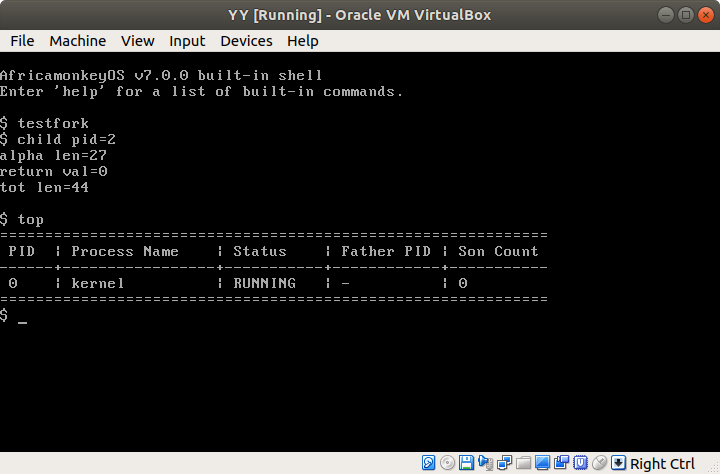
\includegraphics[scale=0.55]{pics/2.png}
\end{figure}

\section{实验总结}

这次实验让我体会到多进程操作系统调试的痛苦!

就是上面遇到的那个问题,我就调了大半天。由于有时钟中断、键盘中断等,我们不能保证每一次程序的执行顺序都是相同的。也许上次能遇到这个 bug ,下一次运行就不能重现。幸运的是,我的程序每次都会跑崩,所以调试相对于刚刚那种情况会简单一些。我能跟踪到子进程的入口地址,查看到子进程的代码段内容,再结合我之前写的代码,就大概能知道怎么回事了。

这个实验也加深了我对进程和线程的理解。我在群里跟凌老师讨论:“我认为 fork 时只复制堆栈是不对的,应该连同代码段、数据段一并复制。因为有些变量不是保存在堆栈,而是数据段。只复制堆栈会导致两个进程共享同一变量。” 凌老师说:“我们的 fork 实质上实现的就是线程。新线程除了 PCB 独立、栈独立,其它的就是要共享!” 我终于明白复制进程是所有段都要复制,而创建线程只需复制堆栈。



\end{document}
















